\documentclass[10pt,a4paper]{article}
\usepackage[utf8]{inputenc}
\usepackage{amsmath}
\usepackage{amsfonts}
\usepackage{amssymb}
\usepackage{graphicx}
\usepackage{hyperref}
\usepackage[font=footnotesize]{caption}
\usepackage{subcaption}
\usepackage{fullpage}
\author{Saulius Lukauskas}
\title{Clustering and Visualisation of DNA Sequencing Data}
\begin{document}
\section{Dataset}
\section{Transcription Starting Sites}
\url{http://encodeproject.org/cgi-bin/hgTables?hgsid=320204017&clade=mammal&org=Human&db=hg19&hgta_group=genes&hgta_track=wgEncodeRegTxn&hgta_table=0&hgta_regionType=genome&position=chr21%3A33%2C031%2C597-33%2C041%2C570&hgta_outputType=wigData&hgta_outFileName=
}

Knownpeaks file has 80922 different entries in the file each corresponding to an unique gene or it's variant.

Note that these entries include some genes in
chromosomes that contain gene contigs in chromosomes that cannot be placed on a specific chromosome,
 annotated as \emph{chrUn} and mappings for a different haplotypes, e.g. \emph{chr6\_cox\_hap6}.
 
These entries will be ignored in datasets like K562 that contain data only for reference regions \emph{chr1--22}, \emph{chrX} and 
\emph{chrM} (mitochondrial DNA).

50659 regions near TSS. in all chromosomes
out of which 48156 have a reference in K562 dataset.

\begin{table}
\begin{tabular}{ll}
\textbf{Reference} & \textbf{Count} \\
\hline
chr1 & 4699 \\
chr2 & 3148 \\
chr19 & 2893 \\
chr11 & 2812 \\
chr17 & 2731 \\
chr6 &  2659 \\
chr3 &  2581 \\
chr7 &  2451 \\
chr15 & 2343 \\
chr12 & 2296 \\
chr5 &  2058 \\
chr9 &  2027 \\
chr16 & 2014 \\
chr10 & 1923 \\
chrX &  1834 \\
chr14 & 1765 \\
chr4 &  1762 \\
chr8 &  1608 \\
chr20 & 1200 \\
chr22 & 1168 \\
chr13 &  846 \\
chr18 &  747 \\
chr21 &  572 \\
chrM &    19 \\
\end{tabular}
\label{table:K562_Regions_of_interest}
\caption{Number of regions of interest in K562 -- not really sure whether they are unique TSS or unique regions}
\end{table}

4 of the regions in this set were invalid, e.g. had start coordinate negative, and thus were just dropped.

Since H3K4Me3 is known to have a distinctive mark around transcription start sites, it is interesting to look at regions around these.

TODO: Explain Transcription start site vs Transcription End Site (negative strand)

I will look at windows of [-2000;+2000) base pairs around the transcription start and end sites. This is similar to approach in TODO: cite some papers.

50659 distinct windows are obtained this way, out of which 48152 correspond to locations in the K562 cell.


\begin{figure}
\centering
\includegraphics[width=0.8\textwidth]{images/read_counts_per_tss_region.eps}
\caption{Figure showing the distribution of read counts falling within a 2000 base pairs window of known TSS locations.}
\label{fig:read_counts_per_tss_region}
\end{figure}

Figure \ref{fig:read_counts_per_tss_region} shows the distribution of read counts falling within a 2000 base pairs window of known TSS locations (Dataset K562, H3K4Me3 Rep1, includes Transcription-end-sites for negative peaks). As one can see from the figure most of the regions of interest have very few reads aligned to them with most regions having 6-7 reads mapped to them. Keep in mind that since the alignments in the data set are all of length of 36bp, we would need at least 112 reads to be able to cover our region of interest with an uniform layer of reads aligned to it. However, we are not interested in covering a region uniformly, and are interested in peaks caused by stacks of reads aligned to the same region.

\begin{figure}
\centering
\begin{subfigure}{0.4\textwidth}
   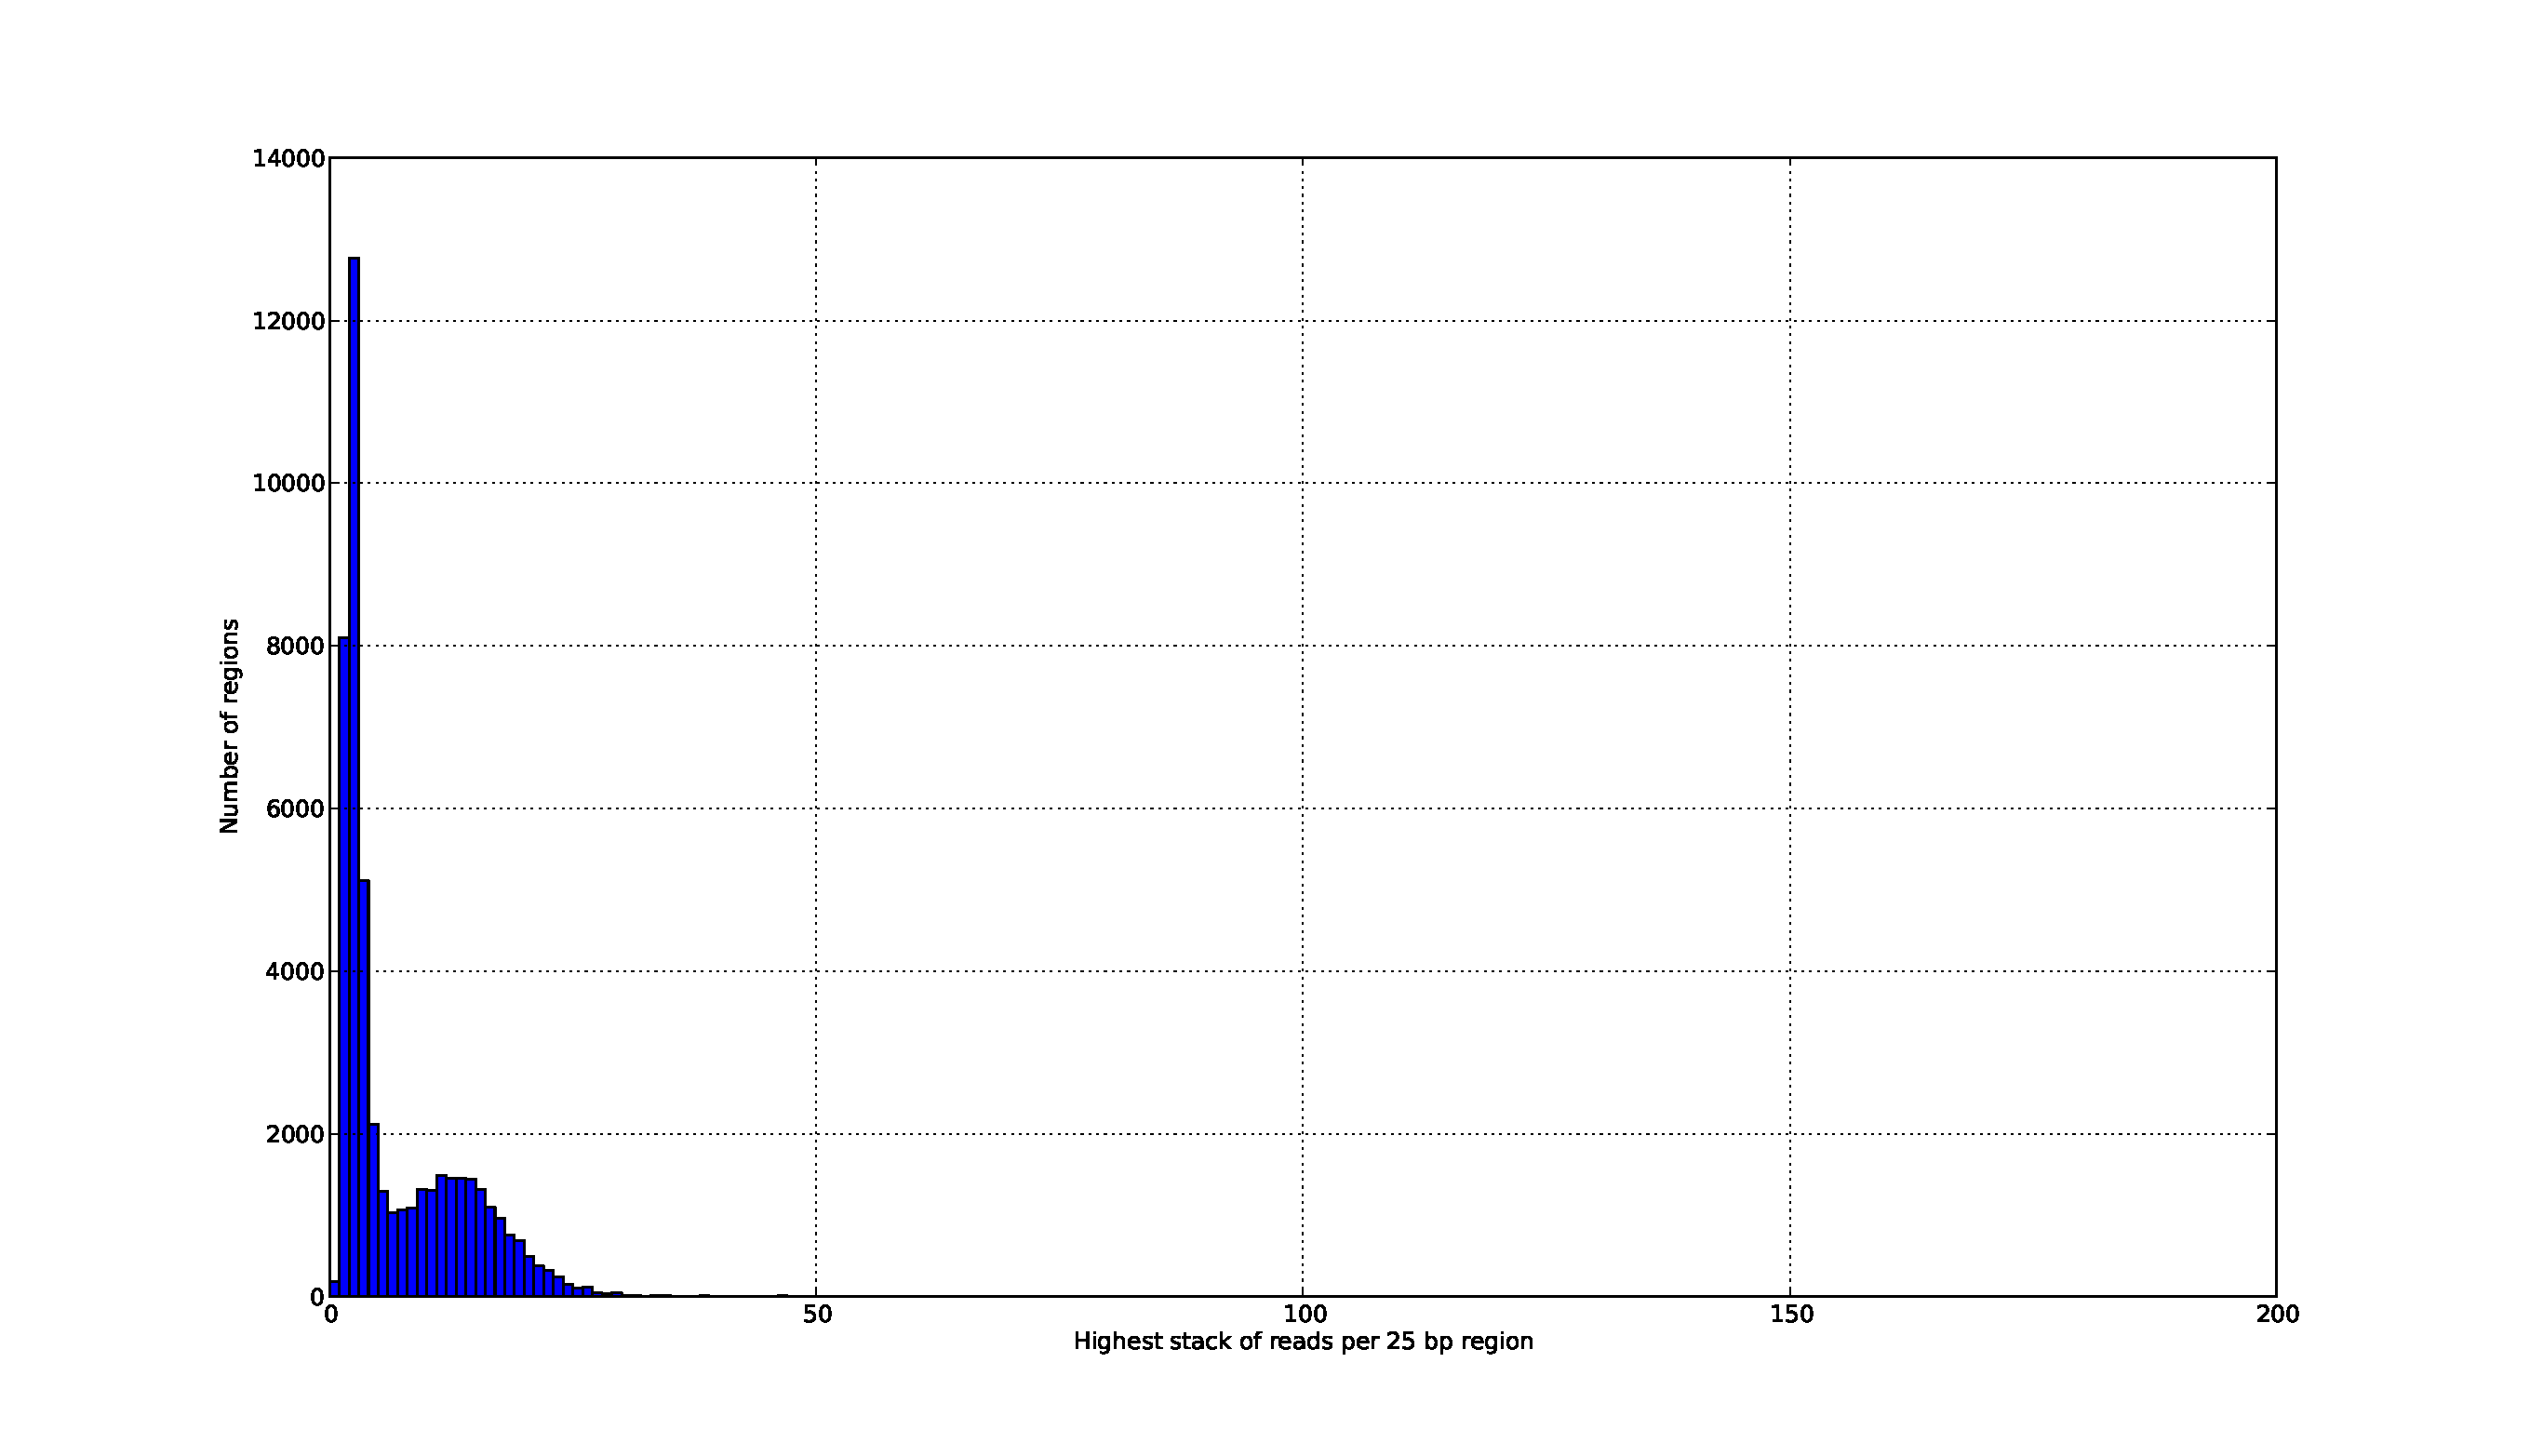
\includegraphics[width=\textwidth]{images/highest_stack.eps}
   \caption{The distribution of highest stacks of reads mapped to regions near TSS}
   \label{fig:highest_stack_distribution}
\end{subfigure}
\begin{subfigure}{0.59\textwidth}
    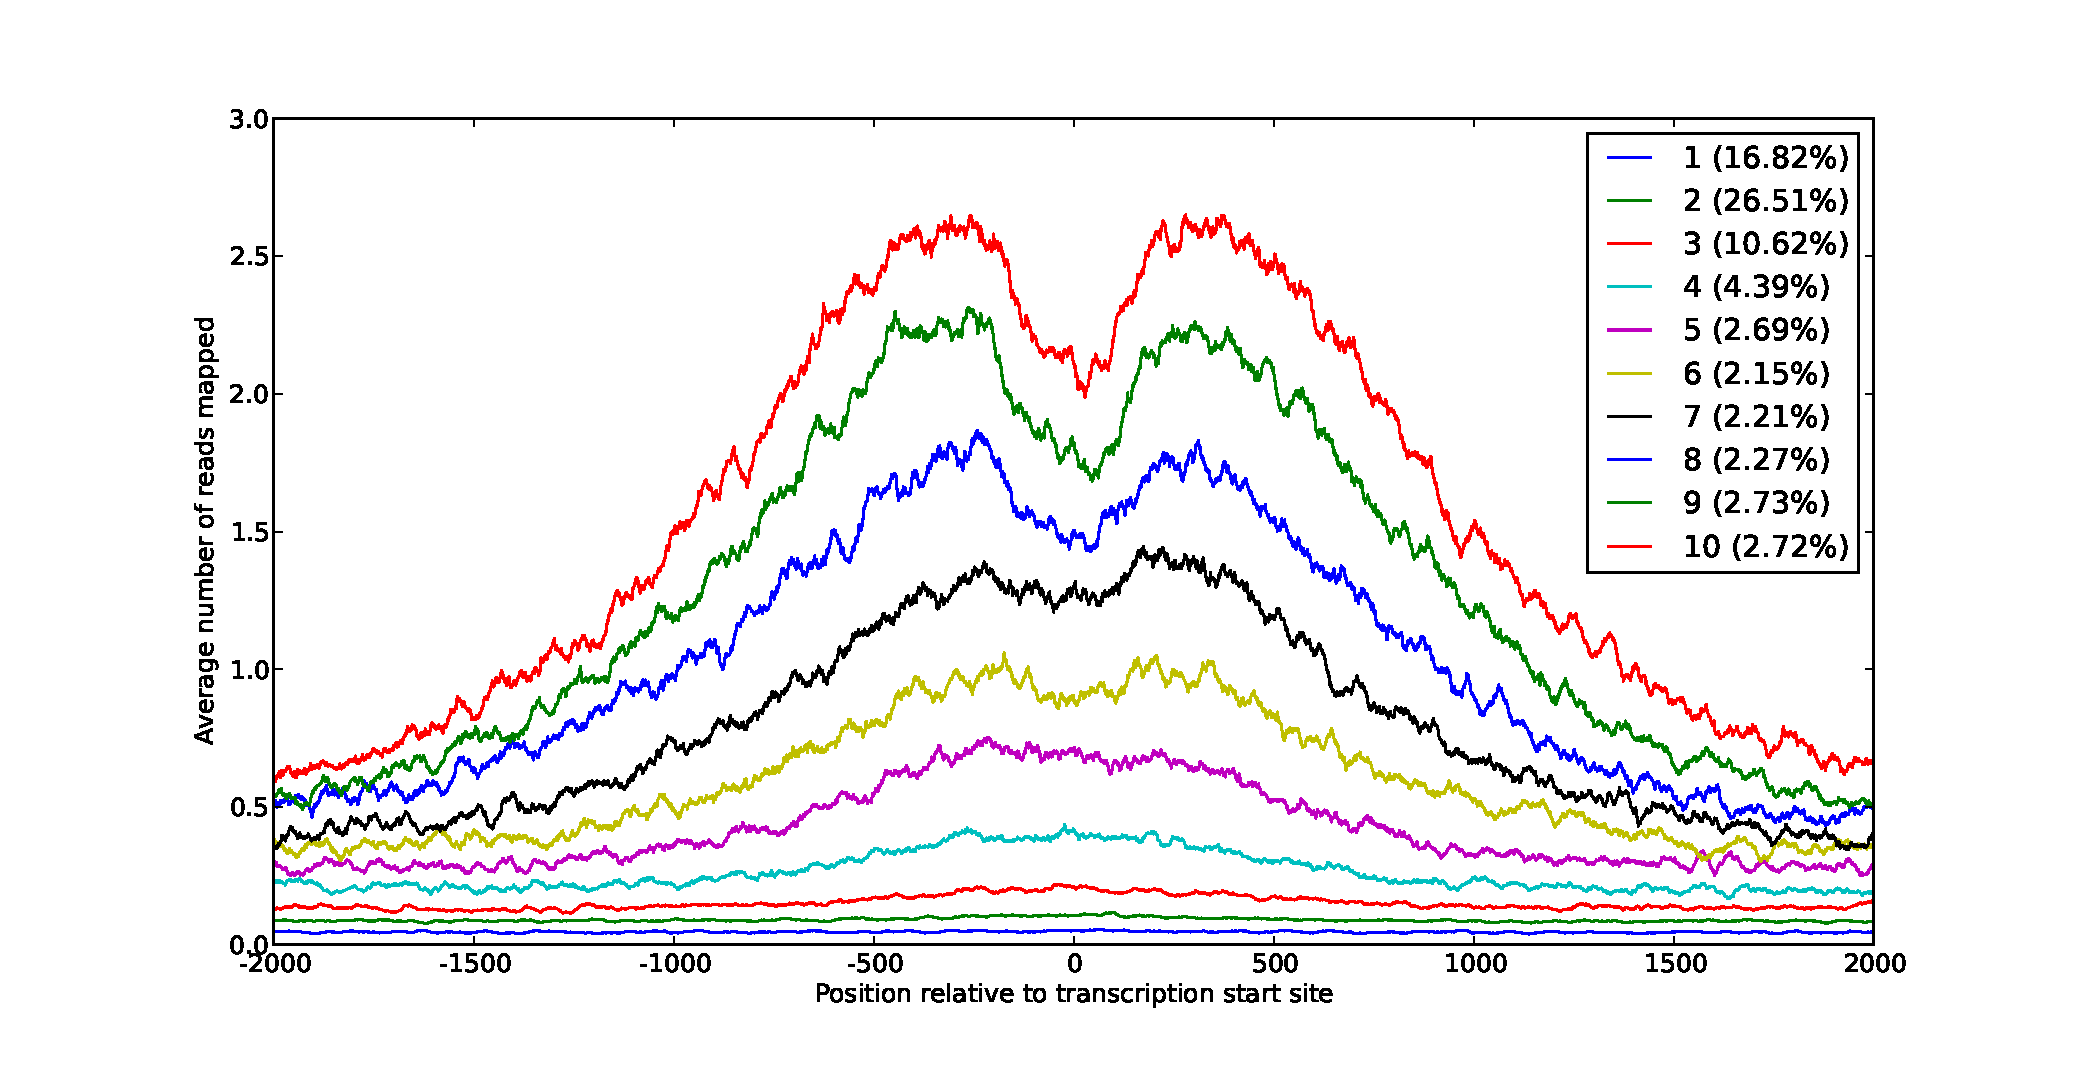
\includegraphics[width=\textwidth]{images/highest_stack_dist_average_marks2.eps}
    \caption{Average H3K4Me3 marks for regions that have highest stacks equal to the numbers in the legend. Numbers in the parentheses show the percentage of items in the dataset with this property.}
    \label{fig:highest_stack_mean_marks}
\end{subfigure}
\caption{Highest stack size distribution and it's related H3K4Me3 marks.}
\label{fig:highest_stacks}
\end{figure}

Figure \ref{fig:highest_stack_distribution} shows the distribution of highest stacks of reads  (i.e. highest column of reads aligned to the same bin) for the dataset. The stacks were calculated by dividing each region into 160 bins of 25 base pairs each and checking how many reads were aligned to these bins. As one can see, the majority of regions have no more than three reads overlapping any of the bins. From figure \ref{fig:highest_stack_mean_marks}, which displays the mean images of regions having their highest columns of sizes between one and ten, we see that the shape of the peak begins to form when four reads overlap at least one bin in the region. The mean marks for the regions that do not have any bins with more than three reads aligned to them are uniform, indicating noise.

Removing the items with highest stacks smaller than three removes 54.33\% of the dataset (including 185 regions that have no reads mapped to them at all). The remaining number of regions of interest around TSS is now 21992.

\begin{figure}
\centering
\begin{subfigure}{0.45\textwidth}
	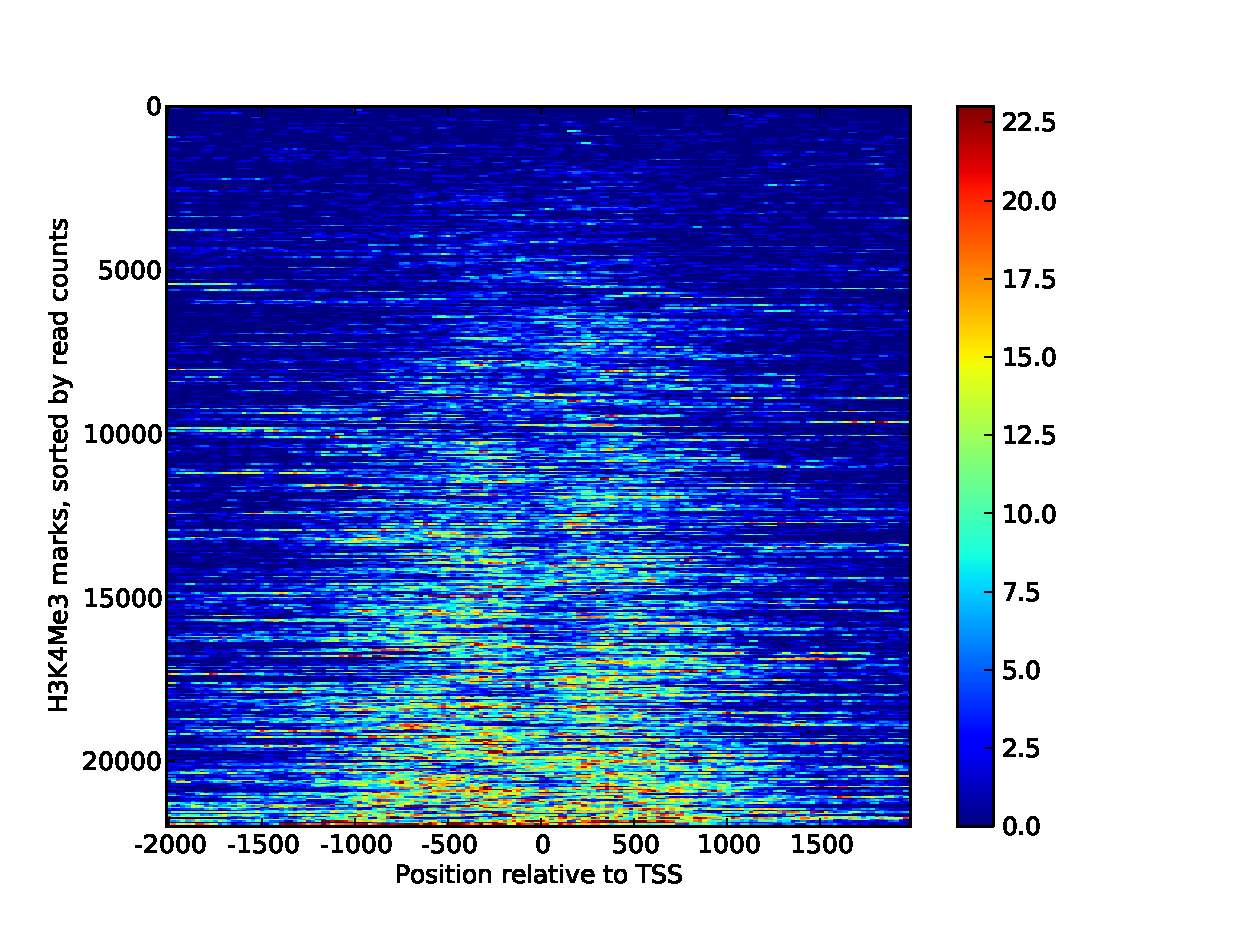
\includegraphics[width=\textwidth]{images/heatmap-k562-h3k4me3-res25-full-peak-data.eps}
	\caption{Heatmap showing unnormalised Data around TSS, resolution 25, H3K4me3, K562}
	\label{fig:heatmap-k562-h3k4me3-unnormalised}
\end{subfigure}
~
\begin{subfigure}{0.45\textwidth}
	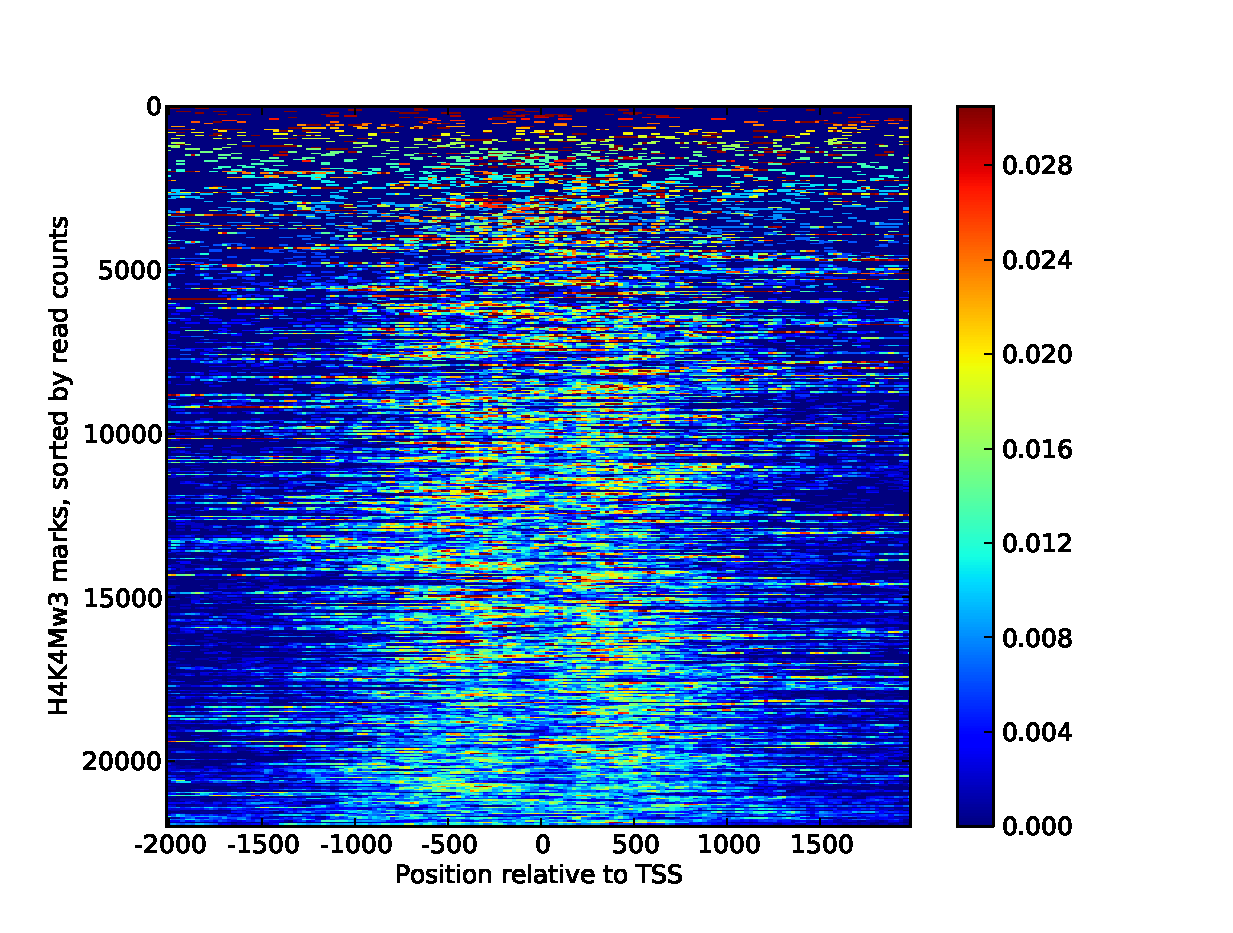
\includegraphics[width=\textwidth]{images/heatmap-k562-h3k4me3-res25-full-normalised-peak-data.eps}
    \caption{Normalised data}
    \label{fig:heatmap-k562-h3k4me3-normalised}
\end{subfigure}
\end{figure}

\subsection{Dynamic Time Warping}

\begin{figure}
\centering
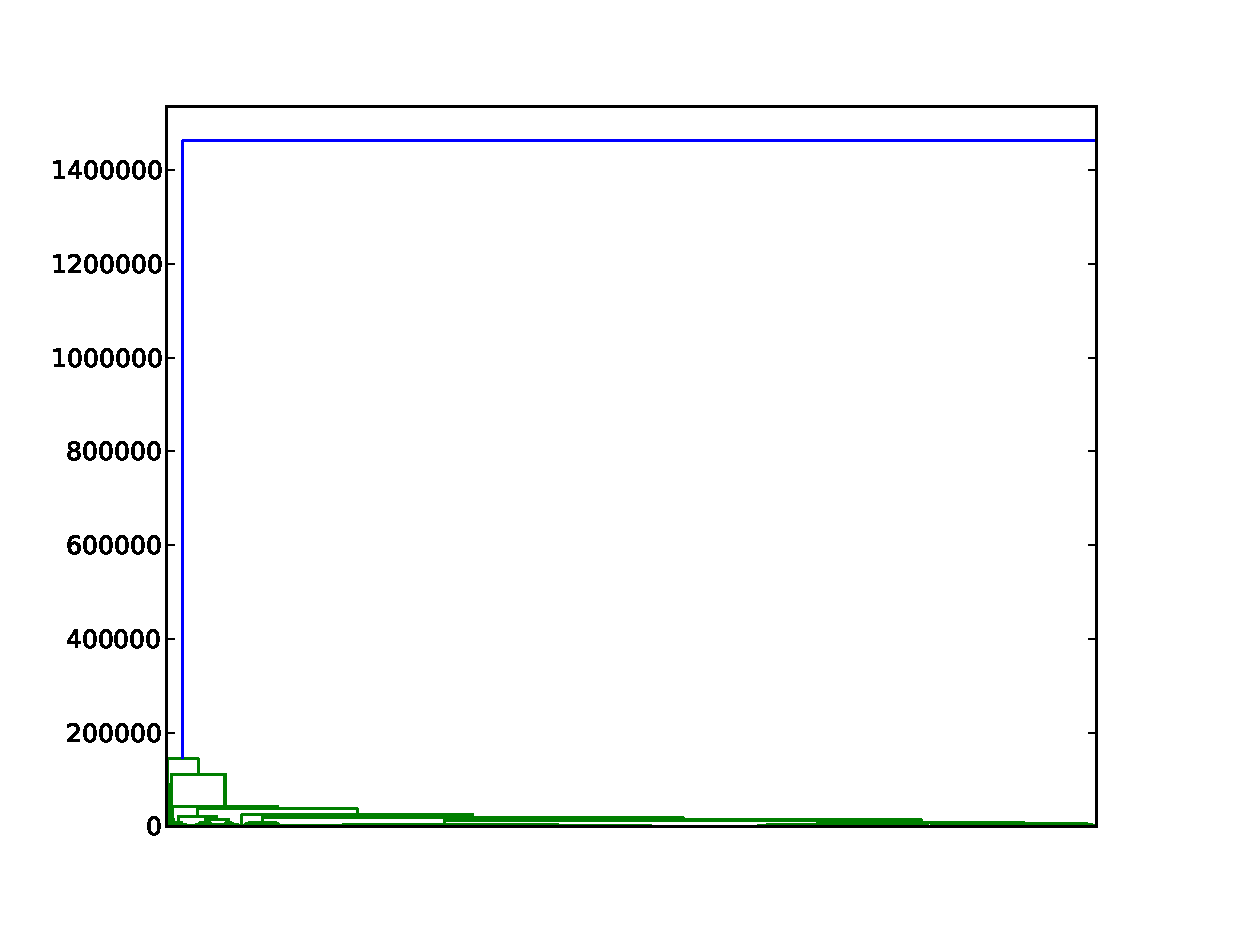
\includegraphics[width=0.5\textwidth]{images/linkage-dtw-std-unnormalised-k562-resolution25.eps}
\caption{Linkage matrix of DTW-std agglomerative clustering distances for TSS dataset, K562, H3K4me3}
\label{fig:linkage-k562-h3k4me3-unnormalised}
\end{figure}

We can see from figure \ref{fig:linkage-k562-h3k4me3-unnormalised} that there is a very odd connection in the linkage matrix that was obtained from unnormalised data.
This connection joins a cluster with a few very highly-expressed peaks with the rest of the data that is expressed much less, showing the sensitivity of DTW for different expression levels.

\begin{figure}
\centering
\begin{subfigure}{0.45\textwidth}
	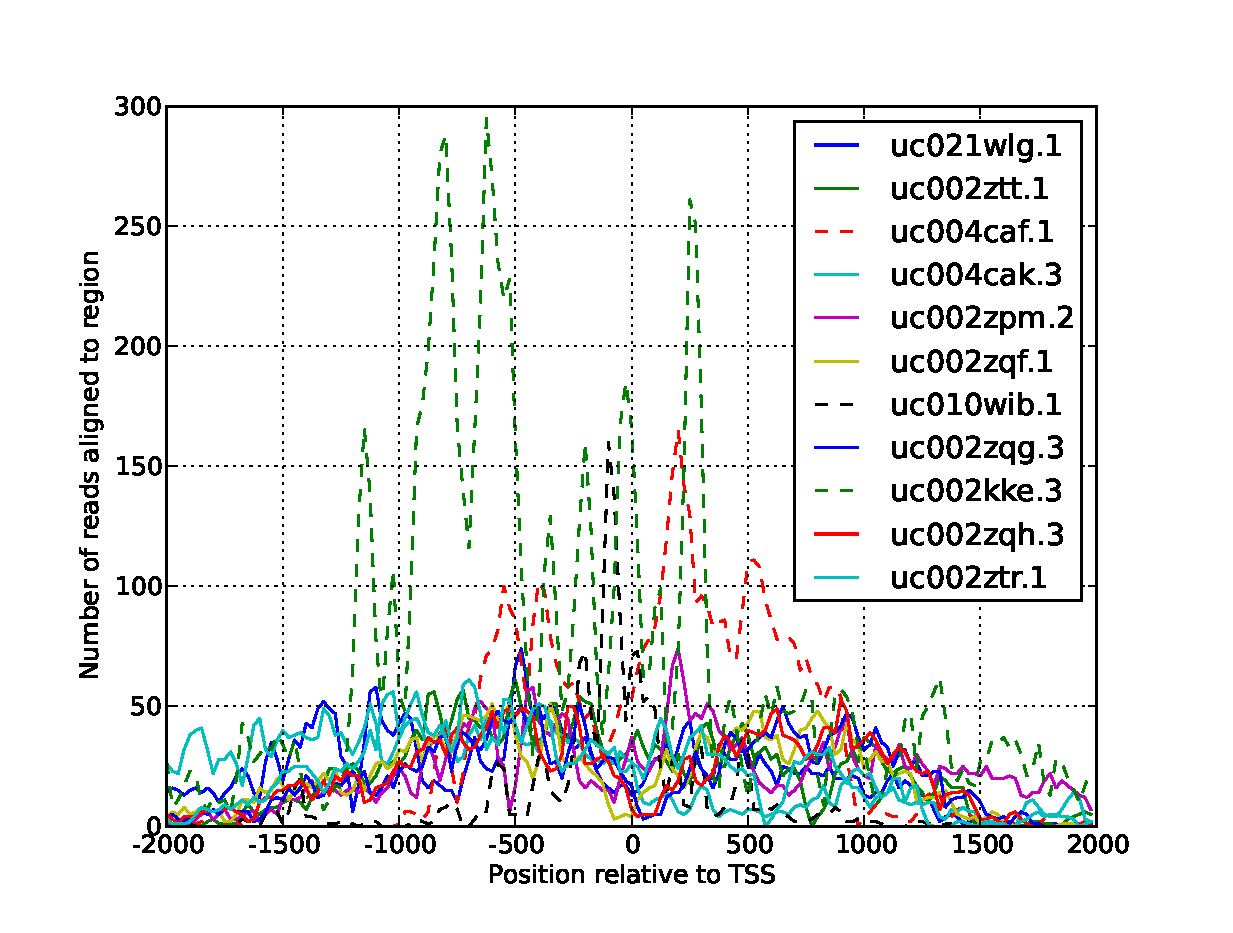
\includegraphics[width=\textwidth]{images/over-expressed-tsses.eps}
	\caption{Unnormalised TSSes}
	\label{fig:oversexpressed-tsses-unnormalised}
\end{subfigure}
~
\begin{subfigure}{0.45\textwidth}
	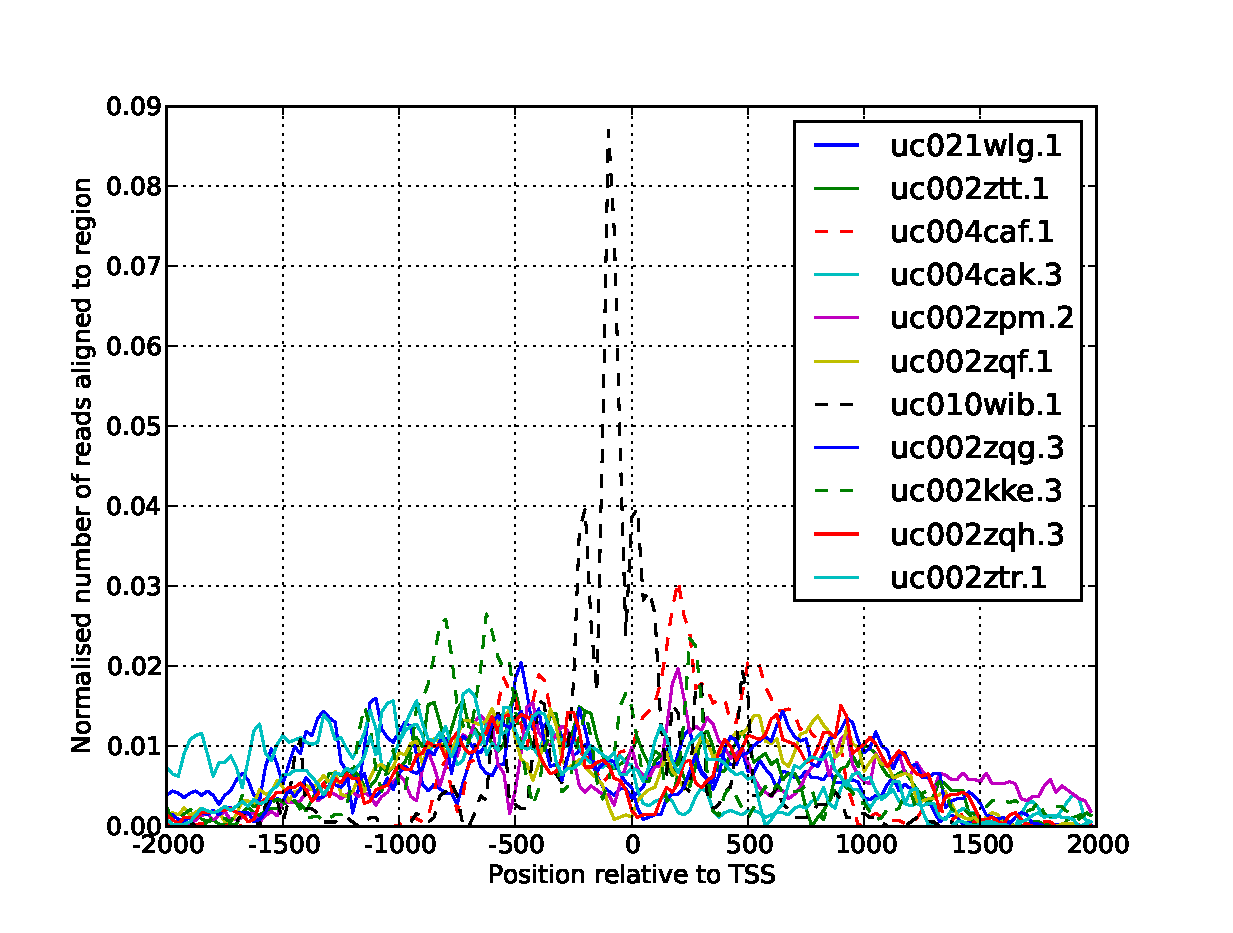
\includegraphics[width=\textwidth]{images/over-expressed-tsses-normalised.eps}
    \caption{Normalised TSSes}
    \label{fig:overexpressed-tsses-normalised}
\end{subfigure}
\caption{TSSes in the cluster joined on the right of linkage matrix in figure \ref{fig:linkage-k562-h3k4me3-unnormalised} (dashed lines) compared to the most expressed peaks in the other cluster before and after normalisation}
\label{fig:overexpressed-tsses}
\end{figure}

Figure \ref{fig:overexpressed-tsses} shows the affects of normalisation for these peaks. Normalisation is done by dividing each peak data by the total read of counts.
We can see that only the pattern around the TSS for gene \verb#uc010wib.1# pops out when the peaks are normalised (figure \ref{fig:overexpressed-tsses-normalised}).
Which is okay because this spike is distinct feature of the shape of the pattern and we indeed want it to stand out.

\subsubsection{Normalised Data Set}

\begin{figure}
\centering
\includegraphics[width=0.5\textwidth]{images/dtw_std-normalised/linkage-dtw-std-normalised-k562-resolution25.eps}
\caption{Linkage matrix obtained from clustering the normalised dataset aggromeratively}
\label{fig:dendrogram-normalised}
\end{figure}

\begin{figure}
\centering
\includegraphics[width=0.5\textwidth]{images/dtw_std-normalised/linkage-k562-split-at-0_2.eps}
\caption{Clusters formed by cutting the dendrogram in \ref{fig:dendrogram-normalised} at 0.2}
\label{fig:dendrogram-normalised-cut-0.2}
\end{figure}

We can see that the linkage matrix obtained by the normalised dataset is easier to interpret. As figure \ref{fig:dendrogram-normalised-cut-0.2} shows, links with high distances now separate noisy regions from the regions with distinctive pattern.

\subsubsection{Sakoe-Chiba band}

\begin{figure}
\centering
\begin{subfigure}{0.45\textwidth}
   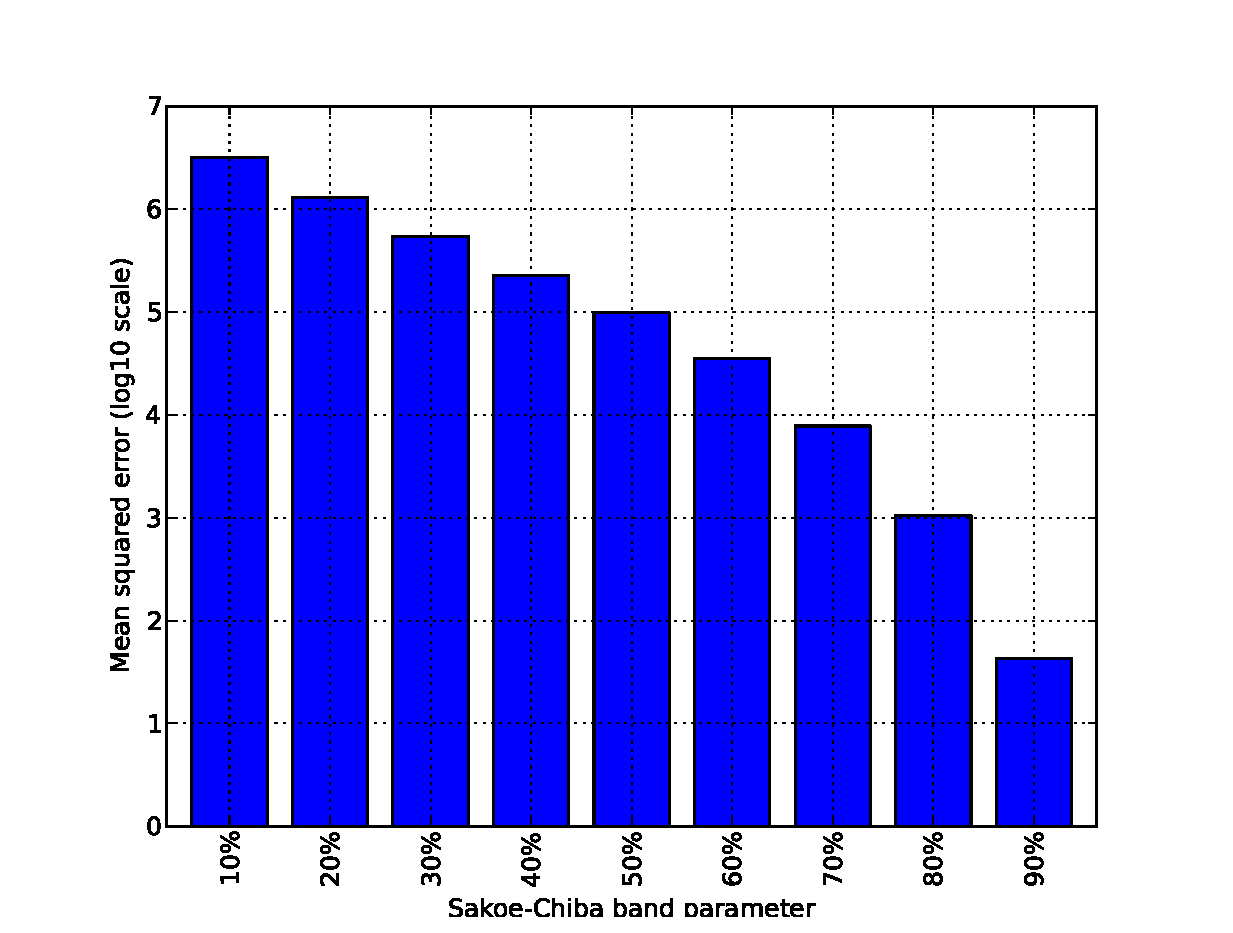
\includegraphics[width=\textwidth]{images/sakoe-chiba-mean-sq-error.eps}
   \caption{Mean squared error of Sakoe-Chiba constraint}
   \label{fig:sakoe-chiba-mean-sq-error}
\end{subfigure}
~
\begin{subfigure}{0.45\textwidth}
    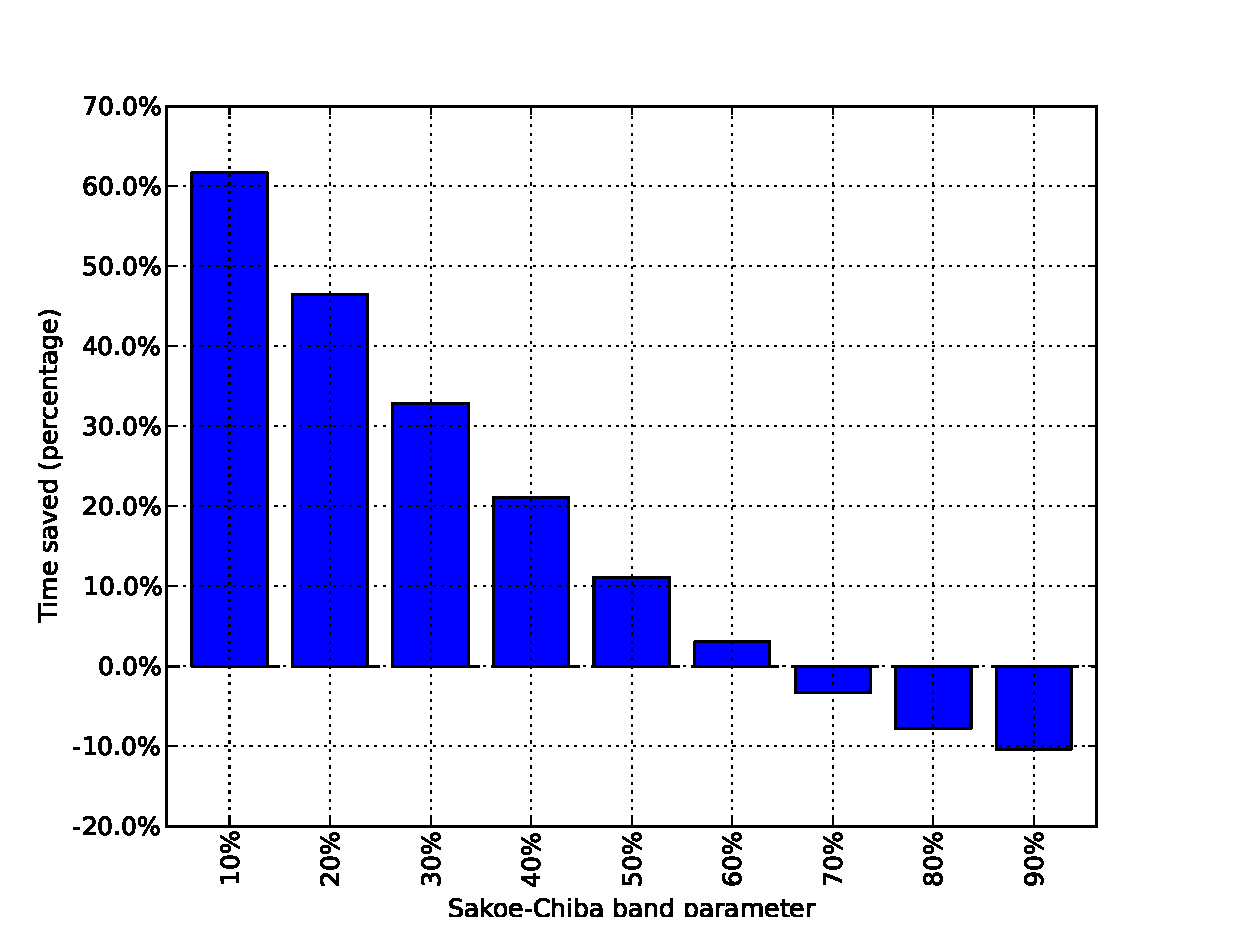
\includegraphics[width=\textwidth]{images/sakoe-chiba-time-saved.eps}
    \caption{Mean saved time (percentage) by Sakoe-Chiba band constraint}
    \label{fig:sakoe-chiba-mean-sq-error}
\end{subfigure}
\label{fig:sakoe_chiba_data}
\caption{Various statistics about Sakoe-Chiba band parameter (estimated from 50 000 random DTW comparisons (resolution 25))}
\end{figure}


\section{Peaks as Points in some N-Dimensional space}
\section{Peaks as Sequential Data}
Euclidean distance is not good for sequential data clustering. (DTW paper)

DTW is mostly used for time data (therefore the name), but can be used for sequential data as well.

DTW algorithm.

Mention that this works for sequences of uneven length.

Outputs of the algorithm and the notion of distance.

DTW is reflexive, symmetric but the triangle equality does not hold.

The complexity of the algorithm, mention that it is unreasonable to use it out of the box.

Ways to reduce complexity: binning, merging points that are equal.

Constraining DTW. 



\subsection{Dynamic Time Warping}
\subsection{Agglomerative Clustering}
\subsection{Prototype Selection}
\subsection{K-Means Clustering}

\bibliographystyle{plain}
\bibliography{papers2}

\end{document}